\documentclass[11pt,a4paper]{article}

\usepackage[margin=2.2cm]{geometry}
\usepackage{times}
\usepackage{amsmath}
\usepackage{booktabs}
\usepackage{graphicx}
\usepackage{xcolor}
\usepackage{tikz}
\usetikzlibrary{arrows.meta,positioning,fit,backgrounds}
\usepackage[colorlinks=true,linkcolor=black,citecolor=black,urlcolor=blue]{hyperref}

\definecolor{imgblue}{HTML}{2878B5}
\definecolor{txtgreen}{HTML}{2A9D6F}
\definecolor{joinred}{HTML}{A61E4D}
\definecolor{warnamber}{HTML}{E67700}
\definecolor{softgray}{HTML}{6C757D}

\newcommand{\code}[1]{\texttt{\small #1}}

\title{\vspace{-1.2cm}\textbf{How the Text Dataset Is Prepared}\\[2pt]
\large A provenance report for the tea pest and disease corpus}
\author{}
\date{}

\begin{document}
\maketitle
\vspace{-1.4cm}

\section*{Summary}

The text side of this project is \textbf{generated, not collected}. No field note
was written by a farmer or an agronomist. Every note is composed by a program
from hand-authored phrase pools, conditioned only on the class label that the
image annotation already carries.

Two separate text corpora exist, produced by two different generators and used
for two different purposes. They must not be confused:

\begin{center}
\small
\begin{tabular}{@{}lll@{}}
\toprule
& \textbf{Corpus A --- crop-linked notes} & \textbf{Corpus B --- symptom bundle}\\
\midrule
File     & \code{tea\_results/annotation/} & \code{data\_final/text\_data/}\\
         & \code{annotations.csv}          & \code{annotations.csv}\\
Generator& \code{backend/tea\_annotator.py} & \code{generate\_tea\_disease\_text()}\\
Rows     & 371 (one per image crop)        & 3{,}000\\
Unique   & 323                             & 673\\
Linked to an image? & Yes, by exact box key & No\\
Used for & the diagnostic model            & the advisory retrieval evaluation\\
\bottomrule
\end{tabular}
\end{center}

\section{Corpus A: the crop-linked field notes}

This is the corpus behind every diagnostic number in the paper. Figure~\ref{fig:pipeline}
shows the pipeline. The image branch and the text branch are produced
independently and then joined on a key that the crop step creates.

\begin{figure}[h]
\centering
\resizebox{\textwidth}{!}{%
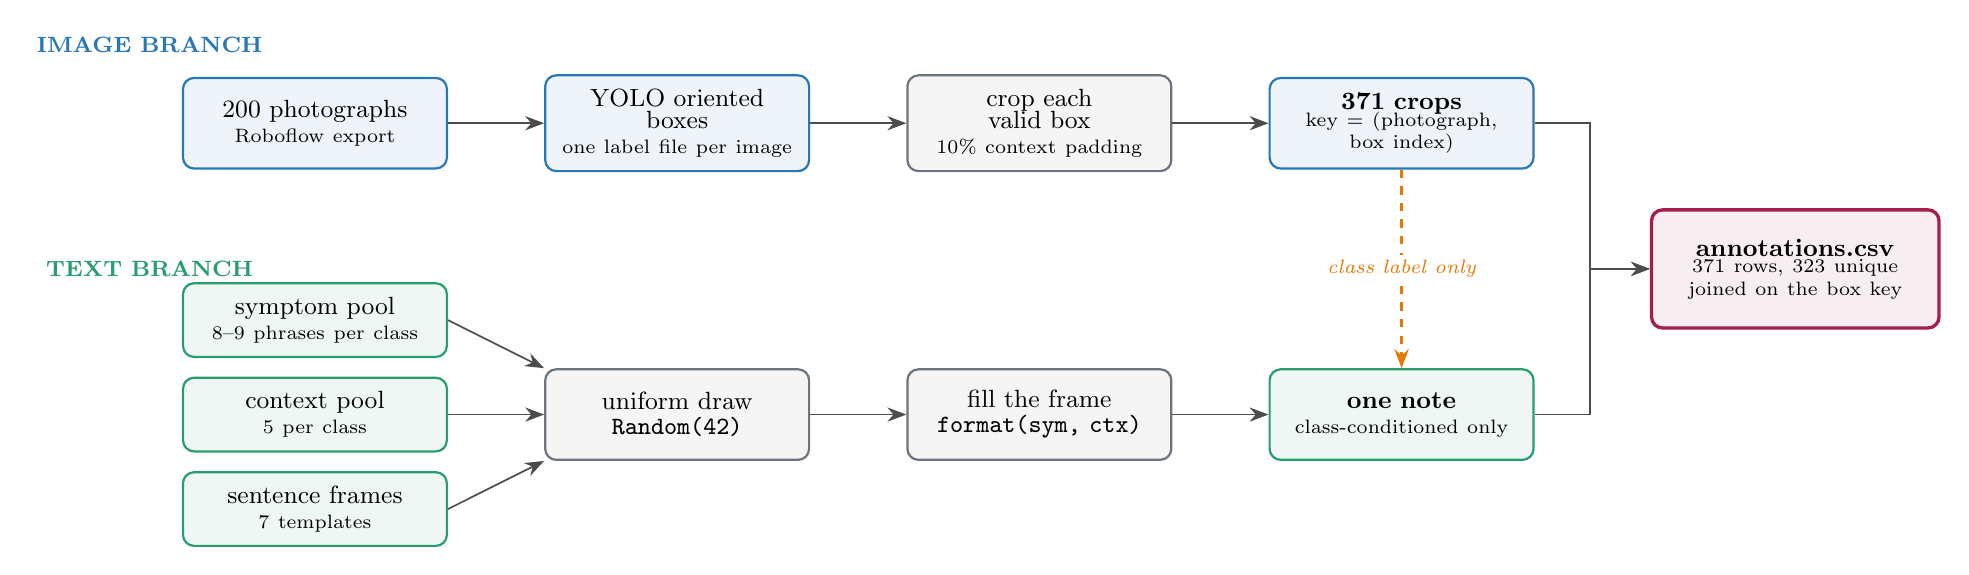
\begin{tikzpicture}[
  font=\small,
  >={Stealth[length=2.4mm]},
  flow/.style={->, semithick, draw=black!70},
  img/.style={draw=imgblue, thick, rounded corners=4pt, fill=imgblue!8,
              align=center, text width=3.0cm, minimum height=1.15cm, inner sep=5pt},
  txt/.style={draw=txtgreen, thick, rounded corners=4pt, fill=txtgreen!8,
              align=center, text width=3.0cm, minimum height=0.85cm, inner sep=5pt},
  op/.style={draw=softgray, thick, rounded corners=4pt, fill=black!4,
             align=center, text width=3.0cm, minimum height=1.15cm, inner sep=5pt},
  merge/.style={draw=joinred, very thick, rounded corners=4pt, fill=joinred!8,
               align=center, text width=3.3cm, minimum height=1.5cm, inner sep=5pt},
  lane/.style={font=\footnotesize\bfseries, align=left}
]

%% Column centres are 4.6cm apart and every box is 3.0cm wide, so no two
%% boxes in a lane can touch.
%% ---- image lane -----------------------------------------------------------
\node[lane, text=imgblue] at (0.3,4.0) {IMAGE BRANCH};
\node[img] (photos) at (2.4,3.0)
  {200 photographs\\[-2pt]\scriptsize Roboflow export};
\node[img] (obb) at (7.0,3.0)
  {YOLO oriented\\[-3pt]boxes\\[-2pt]\scriptsize one label file per image};
\node[op]  (crop) at (11.6,3.0)
  {crop each\\[-3pt]valid box\\[-2pt]\scriptsize 10\% context padding};
\node[img] (crops) at (16.2,3.0)
  {\textbf{371 crops}\\[-2pt]\scriptsize key = (photograph,\\[-3pt]\scriptsize box index)};

\draw[flow] (photos) -- (obb);
\draw[flow] (obb) -- (crop);
\draw[flow] (crop) -- (crops);

%% ---- text lane ------------------------------------------------------------
\node[lane, text=txtgreen] at (0.3,1.15) {TEXT BRANCH};
\node[txt] (sym) at (2.4,0.5)
  {symptom pool\\[-2pt]\scriptsize 8--9 phrases per class};
\node[txt] (ctx) at (2.4,-0.7)
  {context pool\\[-2pt]\scriptsize 5 per class};
\node[txt] (tmpl) at (2.4,-1.9)
  {sentence frames\\[-2pt]\scriptsize 7 templates};

\node[op] (draw) at (7.0,-0.7)
  {uniform draw\\[-2pt]\scriptsize \code{Random(42)}};
\node[op] (fill) at (11.6,-0.7)
  {fill the frame\\[-2pt]\scriptsize \code{format(sym, ctx)}};
\node[txt, minimum height=1.15cm] (note) at (16.2,-0.7)
  {\textbf{one note}\\[-2pt]\scriptsize class-conditioned only};

\draw[flow] (sym.east)  -- (draw.north west);
\draw[flow] (ctx.east)  -- (draw.west);
\draw[flow] (tmpl.east) -- (draw.south west);
\draw[flow] (draw) -- (fill);
\draw[flow] (fill) -- (note);

%% The class label is the only thing that crosses between the two branches.
\draw[flow, dashed, draw=warnamber, very thick] (crops.south) -- (note.north);
\node[font=\scriptsize\itshape, text=warnamber, fill=white, inner sep=2pt]
  at (16.2,1.15) {class label only};

%% ---- merge ---------------------------------------------------------------
\node[merge] (csv) at (21.2,1.15)
  {\textbf{annotations.csv}\\[-2pt]\scriptsize 371 rows, 323 unique\\[-3pt]
   \scriptsize joined on the box key};
\draw[flow] (crops.east) -- ++(0.7,0) |- (csv.west);
\draw[flow] (note.east)  -- ++(0.7,0) |- (csv.west);

\end{tikzpicture}}
\caption{Preparation of the crop-linked corpus. The image branch produces the
pairing key; the text branch never sees the photograph. The dashed arrow is the
only information that crosses between them --- the class label --- which is why
a note describes a \emph{class} rather than the specific leaf it is attached to.}
\label{fig:pipeline}
\end{figure}

\subsection{What the generator actually does}

\code{backend/tea\_annotator.py} holds three hand-authored pools per class and
composes one note per crop:

\begin{center}
\code{sym = rng.choice(\_SYMPTOMS[disease]); ctx = rng.choice(\_CONTEXT[disease]);}\\
\code{tmpl = rng.choice(\_TEMPLATES\_PLAIN); return tmpl.format(symptom=sym, context=ctx)}
\end{center}

\noindent
The draw is seeded with \code{random.Random(42)}, so the corpus is reproducible.
Pool sizes and the resulting combinatorial space are:

\begin{center}
\small
\begin{tabular}{@{}lrrrrr@{}}
\toprule
Class & Symptoms & Contexts & Frames & Distinct notes possible & Crops \\
\midrule
\code{LOOPER\_CATERPILLARS} & 9 & 5 & 7 & 315 & 102\\
\code{LEAF\_BLIGHT}         & 8 & 5 & 7 & 280 & 129\\
\code{LEAF\_HOPPERS}        & 8 & 5 & 7 & 280 & 9\\
\code{LEAF\_RUST}           & 8 & 5 & 7 & 280 & 67\\
\code{MOSQUITO\_BUG}        & 8 & 5 & 7 & 280 & 64\\
\midrule
Total & 41 & 25 & 7 & 1{,}435 & 371\\
\bottomrule
\end{tabular}
\end{center}

\noindent
371 notes are drawn from 1{,}435 possible strings, so collisions occur: the
realised corpus contains \textbf{323 unique texts}, i.e.\ 48 notes are exact
duplicates of another note. A representative row reads:

\begin{quote}\small
\emph{Crop health log: Visible symptom --- irregular brown lesions spreading
along leaf veins with dark borders. Observation context: high humidity and warm
temperatures favoured disease spread.}
\end{quote}

\noindent
which is frame~6 filled with symptom~2 and a matching context string.

\subsection{The unused image-grounded mode}

The same script has an \code{--auto\_caption} mode that runs
\code{Salesforce/blip-image-captioning-base} over each crop and splices the real
caption into five alternative frames. \textbf{The committed corpus does not use
it}: every stored note matches the plain frames, so no image-derived content is
present in the text. This matters --- under the BLIP mode the text would carry
genuine per-leaf visual evidence, and the cross-modal results would mean
something different.

\section{Corpus B: the bundled symptom corpus}

The advisory retrieval evaluation uses a second, independently generated corpus.
Its base pools live in \code{generate\_tea\_disease\_text()}, which holds six
sentences per class and appends, with probability $0.35$, one of four
deliberately ambiguous suffixes such as \emph{``Pattern may overlap with
adjacent stress factors.''} Its stated design goal is the opposite of Corpus A:

\begin{quote}\small
\emph{``Uses purely visual symptom descriptions --- no scientific genus names, no
disease labels embedded in the text. This prevents trivial keyword-matching
shortcuts.''}
\end{quote}

\noindent
Measured directly from the delivered file, the corpus has the following shape:

\begin{center}
\small
\begin{tabular}{@{}lr@{}}
\toprule
Property & Value \\
\midrule
Rows delivered & 3{,}000 (600 per class)\\
Distinct observations & 673\\
Exact duplicate rows & 2{,}327\\
Distinct sentences in the whole corpus & 131\\
Sentences appearing under more than one class & 43\\
Sentences per observation & 2--6 (mean 4.09)\\
Observations with no class-unique sentence & 182 (27.0\%)\\
\bottomrule
\end{tabular}
\end{center}

\noindent
Observations are therefore assembled from a small shared sentence inventory, and
a third of that inventory is not class-specific. This is the direct cause of the
two-regime behaviour reported in the advisory evaluation: retrieval reaches
99.24\% precision@1 on queries carrying at least one class-unique sentence, and
falls to 72.46\% on queries built only from shared sentences.

\section{What this means for the results}

Three consequences follow, and each is stated in the paper rather than left
implicit.

\paragraph{The text-only score is not a language-understanding result.}
Because a note is generated \emph{from} the label, text-only classification is
close to reading the answer back. This is why text-only reaches 96.00\% accuracy
while image-only reaches 61.33\% on the same 75 crops. A 178-token vocabulary of
target-revealing words is fitted on training annotations only and masked
everywhere, which removes explicit disease names, but class-specific symptom
phrasing necessarily remains.

\paragraph{``Exact pairing'' means exact bookkeeping, not co-observation.}
The \mbox{(photograph, box index)} key guarantees that a crop and its note never
land in different splits, which is a real leakage control and an improvement over
the earlier label-aligned proxy pairing. It does not make the note an observation
\emph{of that leaf}. The evidence is in the retrieval numbers: class-level
text-to-image recall@1 is 0.6000 and image-to-text is 0.6133, while
\textbf{exact} text-to-image recall@1 is 1.33\%. The joint space is
class-compatible, not instance-level.

\paragraph{The advisory numbers are upper bounds.}
Corpus B's queries and its retrieval base are disjoint observations but share
sentence vocabulary, so 90.05\% precision@1 should be read as an upper bound
relative to free-form notes.

\section*{Reproducing the corpora}

\begin{quote}
\code{python backend/tea\_annotator.py}\hfill (Corpus A, template mode, seed 42)\\
\code{python backend/tea\_annotator.py --auto\_caption}\hfill (image-grounded mode, unused)\\
\code{python backend/tea\_annotator.py --save\_crops}\hfill (also writes the 371 crop JPEGs)
\end{quote}

\noindent
Corpus B ships pre-generated inside the data bundle. Its base sentence pools
live in

\begin{quote}
\code{backend/FarmFederate\_Colab\_Complete.py}
\end{quote}

\noindent
The exact composer that assembled the delivered multi-sentence observations was
not located in the current tree, so the shape reported in Section~2 is measured
from the delivered file rather than re-derived from source.

\end{document}
